\section{Diskussion}
\label{sec:Diskussion}
Für das Elastizitätsmodul konnten insgesamt vier verschiedene Werte berechnet werden:
\begin{align}
    E_1 &= (120{,}3 \pm 3{,}285) \cdot \mathrm{10^{9}} \frac{\mathrm{N}}{m^2} \\
    E_2 &= (110{,}8 \pm 1{,}753) \cdot \mathrm{10^{9}} \frac{\mathrm{N}}{m^2} \\
    E_3 &= (156{,}6 \pm 8{,}339) \cdot \mathrm{10^{9}} \frac{\mathrm{N}}{m^2} \\
    E_4 &= (100{,}2 \pm 5{,}333) \cdot \mathrm{10^{9}} \frac{\mathrm{N}}{m^2}
\end{align}
Alle Werte bis auf $E_3$ befinden sich im Bereich des Literaturwerts für Kupfer $E_{\mathrm{lit}} = 100 \text{ bis } 130 \cdot \mathrm{10^{9}} \frac{\mathrm{N}}{m^2}$\cite{Kupfer}.
$E_3$ hat eine Abweichung von nur $16,986 \, \%$ zur oberen Grenze des Literaturwerts. So ein kleiner Unterschied kann durch Messfehler oder fehlerhaftes Equipment
hervorgerufen werden. Die zwei verwendeten Messuhren haben teilweise große Differenzen zueinander gehabt. Bei der beidseitigen Einspannung konnte es hier also zu Fehler kommen.\\
Insgesamt befinden sich alle Werte in einem guten Toleranzbereich der Messungenauigkeit. Mithilfe weiterer Messungen an anderen Versuchsaufbauten könnten diese
Messungenauigkeiten noch weiter verringert werden, da dort zum Beispiel ein weiteres Paar Messuhren verwendet werden kann und somit diese Fehlerquelle verringert wird.\\
Das Material kann mit zufriedenstellender Genauigkeit als Kupfer identifiziert werden, da sowohl die Dichte, als auch das Elastizitätsmodul deutlich darauf hinweist. Zudem
konnten die in der Theorie hergeleiteten Gleichungen mit Messdaten verifiziert werden.

\newpage
\section{Originale Messwerte}
\begin{figure}
    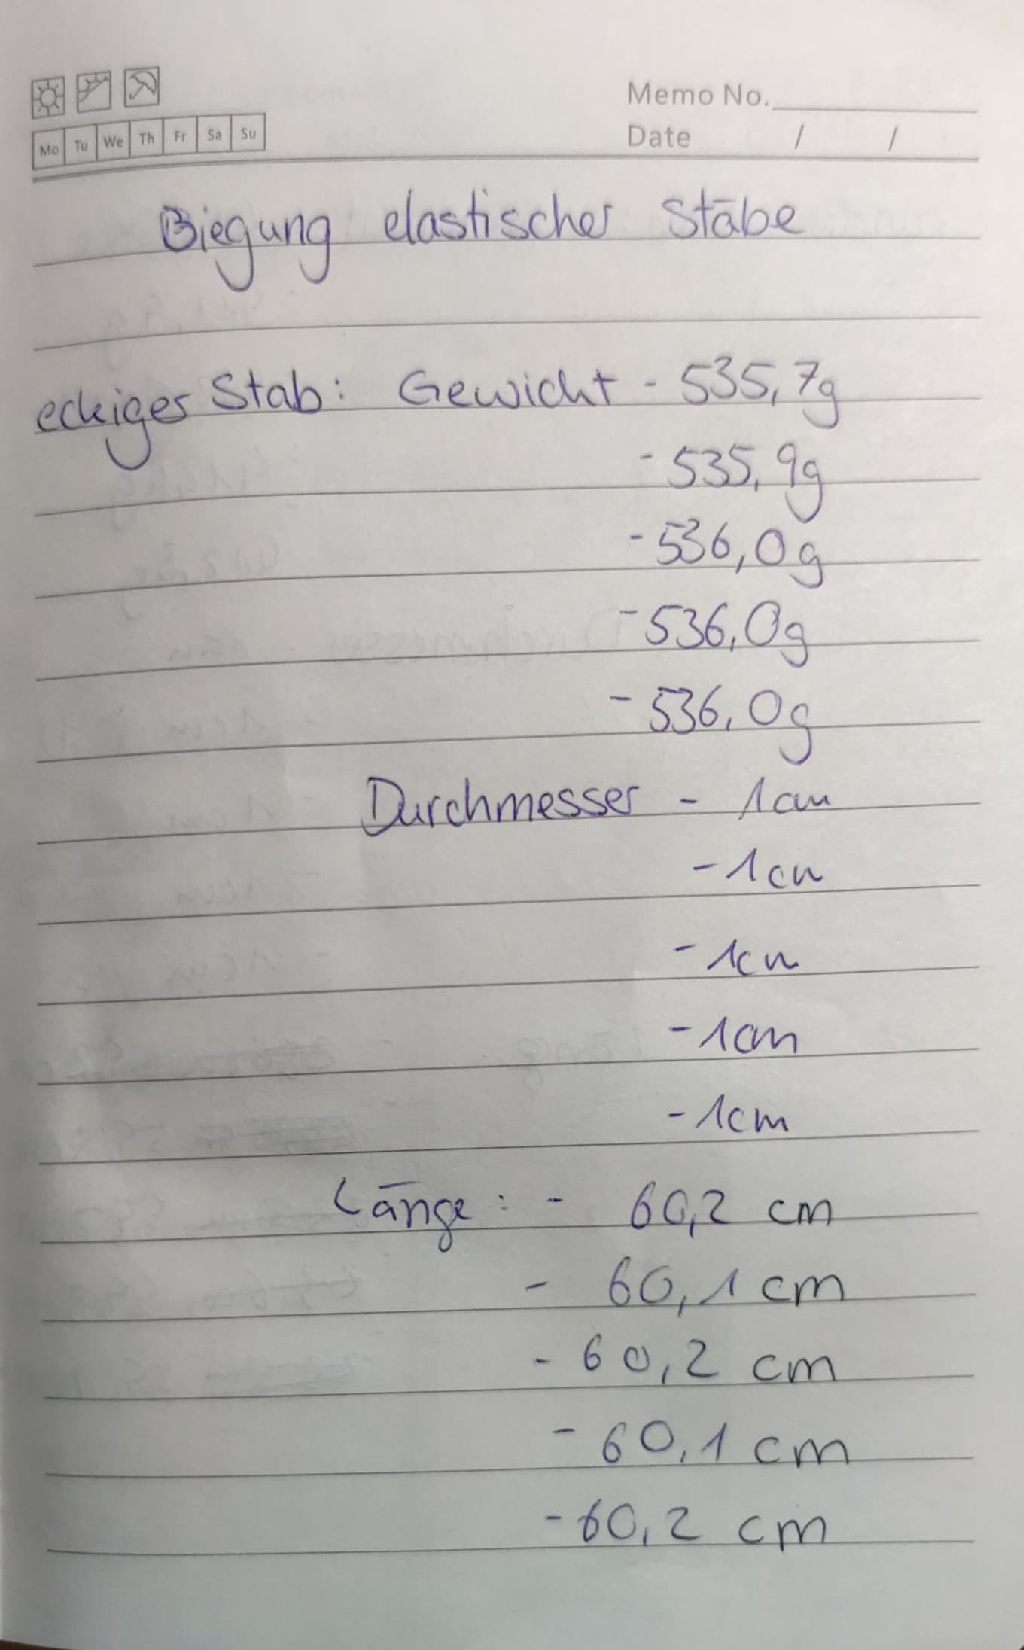
\includegraphics[page=1, width=4.5cm]{Bilder/Messwerte.pdf}
\end{figure}
\begin{figure}
    \includegraphics[page=2, width=9cm]{Bilder/Messwerte.pdf}
\end{figure}
\begin{figure}
    \includegraphics[page=3, width=9cm]{Bilder/Messwerte.pdf}
\end{figure}
\begin{figure}
    \includegraphics[page=4, width=9cm]{Bilder/Messwerte.pdf}
\end{figure}
\begin{figure}
    \includegraphics[page=5, width=9cm]{Bilder/Messwerte.pdf}
\end{figure}
\begin{figure}
    \includegraphics[page=6, width=4.5cm]{Bilder/Messwerte.pdf}
\end{figure}
